\begin{figure}[H]
    \caption{Nodo de caja de selección}
    \centering
    \setlength{\tabcolsep}{0pt}
    \renewcommand{\arraystretch}{1.2}
    \begin{tabular}{
        |>{\centering\arraybackslash}m{(\textwidth - 3\arrayrulewidth) / 2}
        |>{\centering\arraybackslash}m{(\textwidth - 3\arrayrulewidth) / 2}|
    }
        \hline

        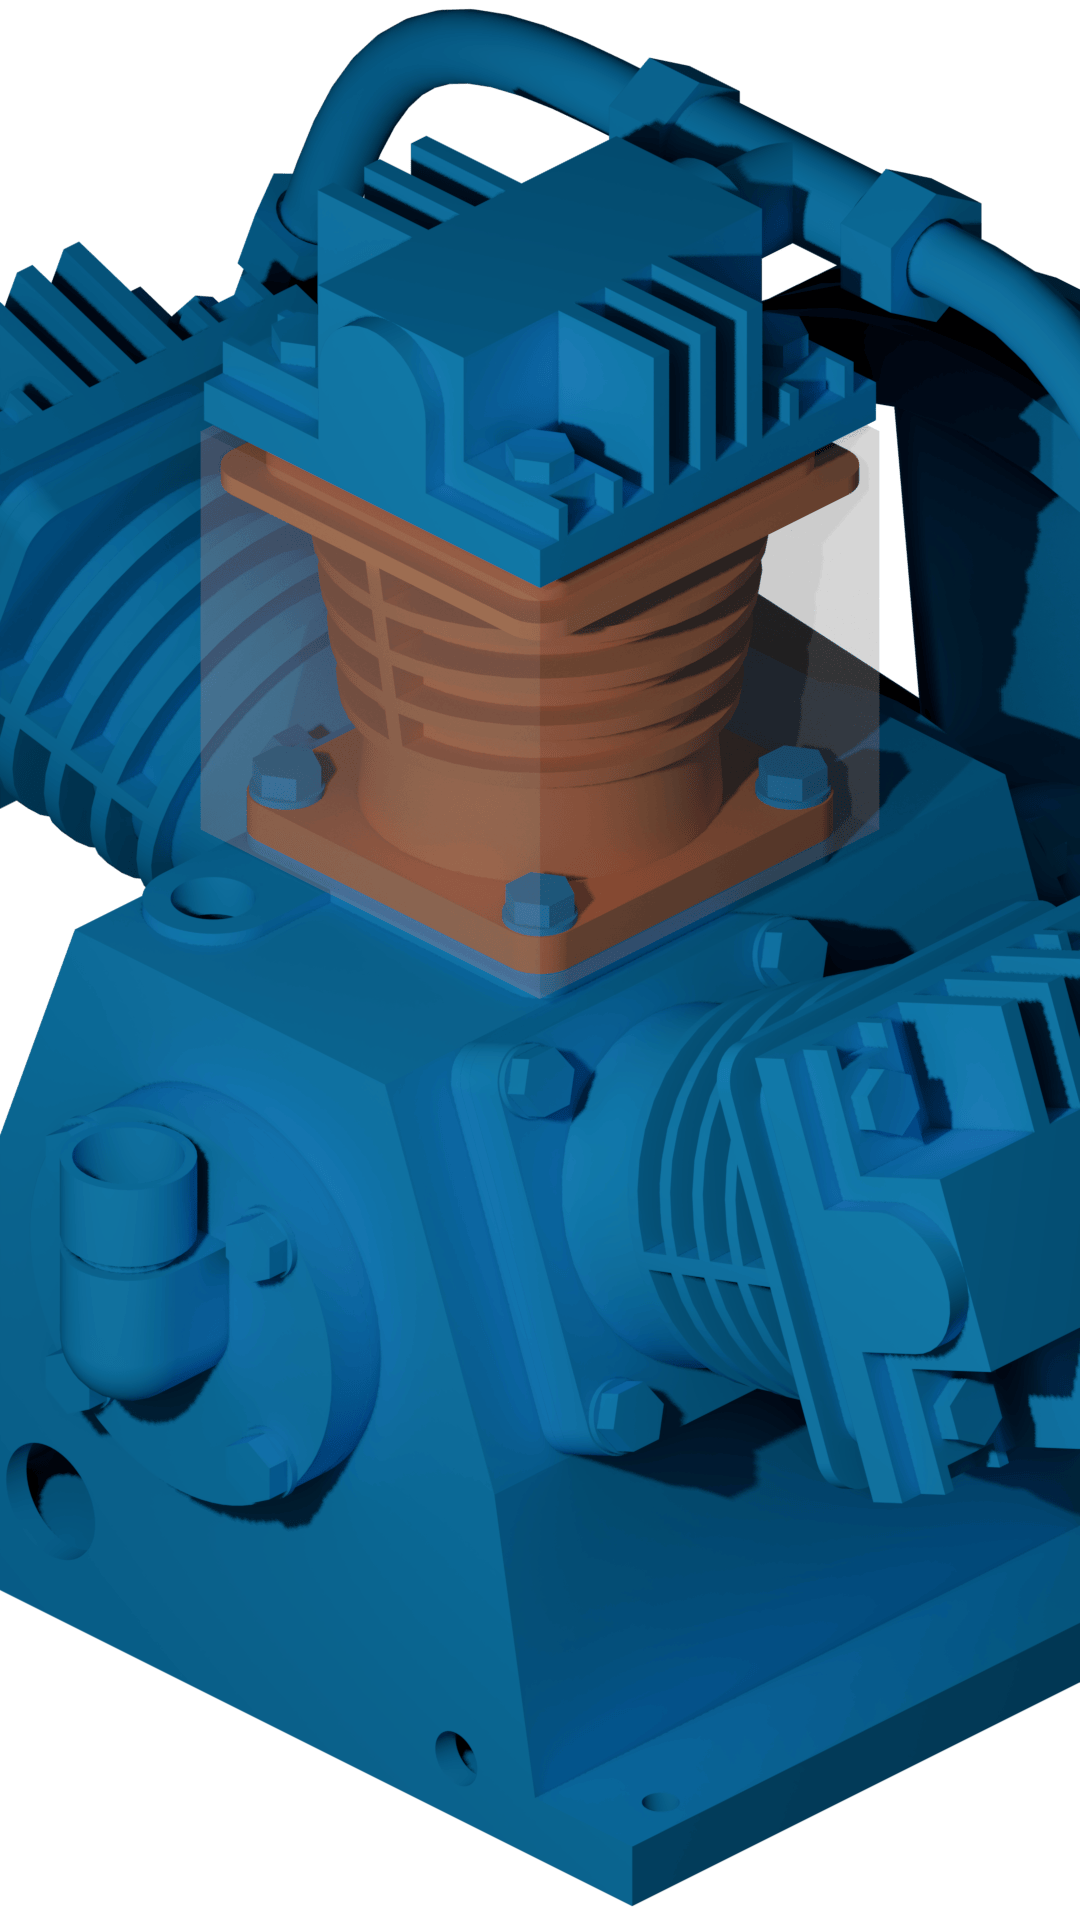
\includegraphics[width=(\textwidth - 3\arrayrulewidth) / 2]
        {assets/figures/second_phase/node/img_node_box_selection.png} &
            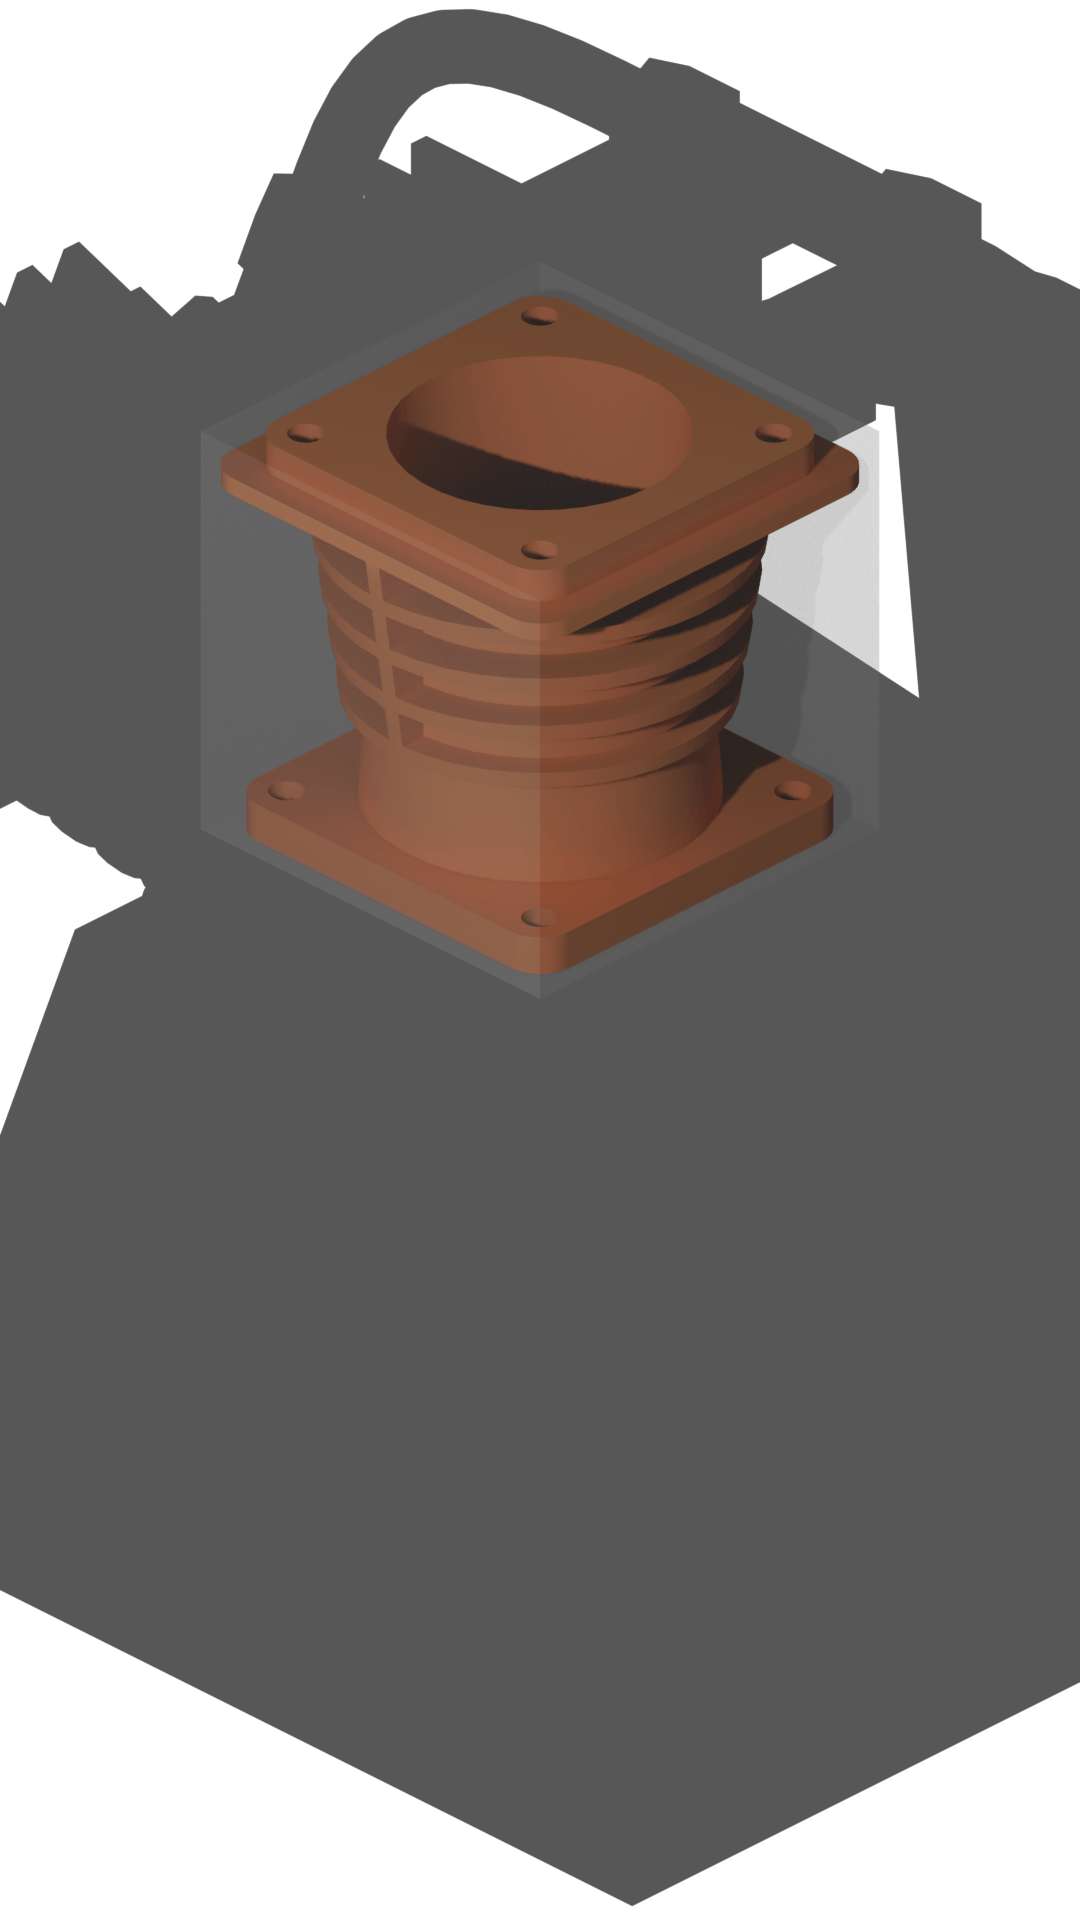
\includegraphics[width=(\textwidth - 3\arrayrulewidth) / 2]
        {assets/figures/second_phase/node/img_node_box_isolated.png} \\

        \small Selección de submodelo &
            \small Selección de submodelo aislada \\
        
        \hline
    \end{tabular}
    \label{fig:node_box}
\end{figure}
\fixvspace{0}